%% Chapter 11 — Bill of Materials & Procurement
%% Course 247-519-VA, Vanier College
%% Project Planning & Prototyping

\chapter{Bill of Materials \& Procurement}
\label{ch11}

\paragraph{Where this fits.}
This chapter operates at Stage~3 (Development), targeting Gate~3.
The Stage-Gate model requires that every Gate~3 review package include a
\emph{costed} BOM: a document that ties every physical part to a quantity, a
unit price, a supplier, and a lead time.
An uncosted or incomplete BOM cannot support the business case that Gate~3
demands --- no reviewer can approve a prototype budget without knowing what it
costs to build.

\paragraph{Learning Objectives.}
After completing this chapter you will be able to:
\begin{enumerate}
  \item Build a multi-level costed BOM with correct reference designators,
        quantities, unit costs, extended costs, and supplier information.
  \item Derive a purchase list from the BOM and compare supplier quotes on both
        unit price and lead time.
  \item Manage the full procurement document chain: purchase order, receipt,
        invoice verification, and as-built reconciliation.
\end{enumerate}

Knowing \emph{when} work happens (the Gantt chart from Chapter~10) and what could go wrong (the risk register) is only actionable once you know what to order, from whom, at what price, and within what lead time. This chapter provides that foundation.

% ─────────────────────────────────────────────────────────────────────────────
\section{BOM as a Design Document}
\label{sec:ch11-bom-design}
% ─────────────────────────────────────────────────────────────────────────────

A \textbf{bill of materials}\index{bill of materials} (BOM) is not a shopping
list.
It is a design document that captures the complete set of physical parts
required to build one unit of the system, together with the quantities,
reference designators, unit costs, and supply-chain metadata necessary to
procure and assemble those parts.
The distinction matters: a shopping list can be incomplete without consequences
until you arrive at the checkout; an incomplete BOM discovered during assembly
halts production, delays the schedule, and invalidates cost estimates already
submitted to the Gate~3 review.

\subsection{BOM Levels}
\label{sec:ch11-bom-levels}

A \textbf{multi-level BOM}\index{bill of materials!multi-level} structures the
system hierarchically: the top level names the assembled product; the second
level names subsystems or subassemblies; the lowest level names individual
purchased or manufactured components.
This structure mirrors the system architecture developed in Chapter~5 and makes
it possible to roll costs up by subsystem, identify which assembly contributes
most to total cost, and manage procurement independently for each assembly team.

Figure~\ref{fig:ch11-bom-tree} shows the multi-level BOM tree for the IoT
robotic sorting subsystem.
The top level is the complete sorter.
The second level contains three subsystems: Control, Actuation, and Structure.
The third level contains the individual line items.

\begin{figure}[htbp]
  \centering
  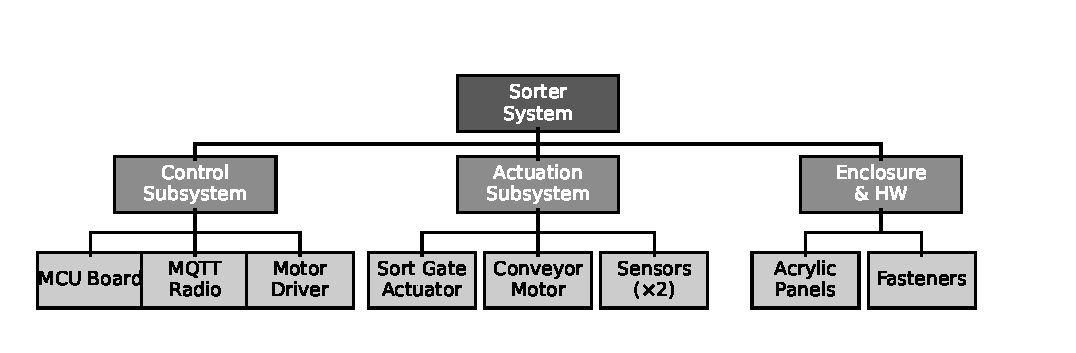
\includegraphics[width=0.88\textwidth]{images/fig_02_bom_tree}
  \caption{Multi-level BOM tree for the IoT robotic sorting subsystem.
           The top-level assembly (Sorter) decomposes into three subsystems
           (Control, Actuation, Structure), each of which decomposes into
           individual purchased components at Level~3.
           Reference designators (U1, U2, Q1, M1, B1, B2, H1) appear at the
           leaf nodes.}
  \label{fig:ch11-bom-tree}
\end{figure}

\subsection{BOM Fields}
\label{sec:ch11-bom-fields}

Every BOM line requires at minimum:

\begin{enumerate}
  \item[(a)] \textbf{Reference designator}\index{reference designator} ---
        the unique identifier linking the BOM line to the schematic or assembly
        drawing (e.g., U1, Q1, M1).
        A line without a designator cannot be placed on a board or found in an
        assembly drawing.

  \item[(b)] \textbf{Description and part number} --- the manufacturer part
        number (MPN) is the only unambiguous identifier.
        A description without an MPN allows the assembler to substitute any
        part that ``sounds like'' the intended one.

  \item[(c)] \textbf{Quantity per assembly} ($q_i$) --- the number of that
        part needed to build one unit.

  \item[(d)] \textbf{Unit cost} ($u_i$, in CAD) --- the price paid per single
        piece at the procurement quantity.

  \item[(e)] \textbf{Extended cost} --- $q_i \times u_i$, the total spend on
        that line for one assembly.

  \item[(f)] \textbf{Preferred supplier and part number} --- the distributor
        from whom the part will be ordered, with the distributor's stock number.

  \item[(g)] \textbf{Lead time} --- the calendar days from order placement to
        receipt, used to back-schedule the procurement milestone in the Gantt
        chart.

  \item[(h)] \textbf{Alternate part} --- a second-source MPN that satisfies
        parametric equivalence and footprint compatibility, mitigating
        single-source risk identified in the risk register.
\end{enumerate}

\paragraph{In Practice.}
A team building the sorter prototype omitted reference designators from the BOM
because the schematic had not been finalised when the BOM was started.
At assembly, the PCB had two footprint-compatible motor drivers with different
pinouts.
Without the designator, the assembler soldered the wrong driver onto U2, applying
power in the wrong sequence and destroying the part.
The loss was \$18 and two days of schedule.
Reference designators must be locked before the BOM is submitted, not after.

\subsection{The Alternate-Part Column}
\label{sec:ch11-alternates}

Single-sourced components\index{single-source risk} are a procurement liability.
If the sole supplier for a critical part is out of stock, the project stalls.
Every BOM line for a component that is not a commodity (i.e., not a standard
resistor, capacitor, or fastener available from every distributor) should carry
a vetted alternate: a second MPN confirmed to be parametrically equivalent,
footprint-compatible, and in Active lifecycle status.
Chapter~6 described the process for qualifying a second source; the BOM is
where that work is recorded and made visible to reviewers.

% ─────────────────────────────────────────────────────────────────────────────
\section{Purchase List from BOM}
\label{sec:ch11-purchase-list}
% ─────────────────────────────────────────────────────────────────────────────

A \textbf{purchase list}\index{purchase list} is derived from the BOM by
collapsing identical MPNs that appear in different subsystems into a single
line and then computing the order quantity for each line.
The purchase list is the document you send to a supplier or purchasing
department; it is not the BOM itself.

\subsection{Order Quantity with Overage}
\label{sec:ch11-order-qty}

For passive components and consumables --- resistors, capacitors, solder,
heat-shrink --- the risk of loss during assembly justifies ordering more than
the exact quantity the BOM requires.
The \textbf{order quantity with overage}\index{order quantity!overage} is:

\begin{equation}\label{eq:ch11-order-qty}
  q_i^{\text{order}} = \left\lceil (1 + \alpha)\,q_i \right\rceil
\end{equation}

where $q_i$ is the BOM quantity, $\alpha$ is the fractional overage
(a dimensionless value between 0 and 1, e.g., $\alpha = 0.10$ for 10\,\%
overage), and $\lceil\,\cdot\,\rceil$ denotes the ceiling function (round up
to the nearest whole unit).
The ceiling is necessary because you cannot order a fractional part.

Overage is \emph{not} applied blindly to every line.
Expensive unique components --- the MCU board, the motor driver IC, the
enclosure --- are ordered to exact BOM quantity, possibly with one spare unit
explicitly approved by the project manager.
Applying 10\,\% overage to a \$65 MCU board would order an unneeded extra unit
and misrepresent the budget.

\paragraph{Common Pitfalls.}
Teams sometimes apply overage to the BOM quantity used for cost estimation,
inflating $C_{\text{BOM}}$.
Overage belongs only on the purchase list, applied to $q_i^{\text{order}}$;
the BOM cost calculation always uses the exact per-assembly quantity $q_i$.

% ─────────────────────────────────────────────────────────────────────────────
\section{Quotes and Supplier Comparison}
\label{sec:ch11-quotes}
% ─────────────────────────────────────────────────────────────────────────────

A \textbf{request for quotation}\index{request for quotation} (RFQ) specifies the MPN, the order quantity, the required delivery date, and the delivery address; send one to at least two suppliers for every non-commodity line item before committing to a purchase order.

\subsection{What to Compare}
\label{sec:ch11-quote-compare}

Quote comparison is not a simple lowest-price sort.
The relevant criteria are:

\begin{enumerate}
  \item[(a)] \textbf{Unit price at your order quantity} --- distributor pricing
        is typically tiered; the unit price at quantity~1 may be three times
        the price at quantity~10.
        Always quote at the quantity you intend to order.

  \item[(b)] \textbf{Lead time} --- a part that is \$2.00 cheaper but arrives
        four weeks later may miss the assembly milestone and delay Gate~3.
        Lead time must be evaluated against the Gantt chart, not in isolation.

  \item[(c)] \textbf{Stock availability} --- a listed unit price is irrelevant
        if the distributor has zero units in stock.
        Confirm ``in-stock'' quantity at time of RFQ.

  \item[(d)] \textbf{Minimum order quantity} (MOQ) --- some distributors impose
        a minimum order of 5 or 10 units for certain components.
        The effective cost per unit changes when the MOQ exceeds your order
        quantity.

  \item[(e)] \textbf{Shipping and handling} --- a \$1.50 unit price advantage
        is erased by a \$15 shipping surcharge on a small order.
\end{enumerate}

The procurement document chain that connects the BOM to payment is shown in
Figure~\ref{fig:ch11-doc-chain}.

\begin{figure}[htbp]
  \centering
  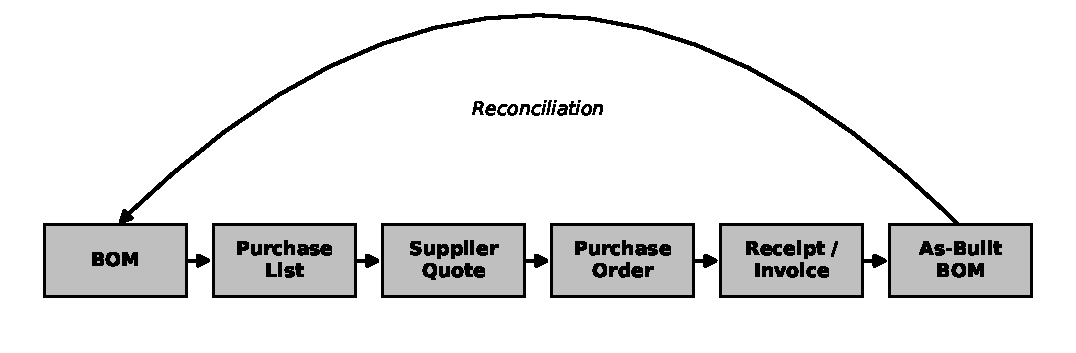
\includegraphics[width=0.95\textwidth]{images/fig_01_doc_chain}
  \caption{Procurement document chain for the sorter prototype.
           Flow proceeds left to right: the costed BOM feeds the purchase list;
           the purchase list generates RFQs to suppliers; selected quotes become
           purchase orders (POs); POs trigger shipments that produce a packing
           slip and invoice; receipt verification produces the as-built BOM
           through reconciliation.
           Each arrow represents a document hand-off with a defined format and
           responsible party.}
  \label{fig:ch11-doc-chain}
\end{figure}

% ─────────────────────────────────────────────────────────────────────────────
\section{Purchase Orders}
\label{sec:ch11-po}
% ─────────────────────────────────────────────────────────────────────────────

A \textbf{purchase order}\index{purchase order} (PO) is a formal document that
authorises a supplier to ship specific goods at a specific price.
It is a legal instrument: once a supplier accepts a PO, both parties are bound
by its terms.
For student projects, purchase orders are often replaced by a supervisor-approved
purchase requisition or a direct online order; the discipline of treating that
order as a PO --- with a unique PO number, a line-item list, and a price
commitment --- is nonetheless valuable and expected in industry.

\subsection{Required PO Fields}
\label{sec:ch11-po-fields}

A well-formed PO contains:

\begin{enumerate}
  \item[(a)] \textbf{PO number} --- a unique identifier used to cross-reference
        the invoice and packing slip.
  \item[(b)] \textbf{Issue date and required-by date}.
  \item[(c)] \textbf{Line items}: supplier part number, MPN, description, ordered
        quantity, agreed unit price, and line total.
  \item[(d)] \textbf{Ship-to address} and delivery instructions.
  \item[(e)] \textbf{Payment terms} (e.g., Net 30, credit card on shipment).
  \item[(f)] \textbf{Authorising signature or approval} --- in a student lab
        context, this is the instructor or technician approval on the
        requisition form.
\end{enumerate}

\paragraph{In Practice.}
PO numbers serve a critical traceability function.
When two packages arrive on the same day from the same distributor, the packing
slip PO reference is the only reliable way to match each package to its
originating order without opening and counting every item.
Assign PO numbers sequentially from the project start and record them in the
procurement log.

% ─────────────────────────────────────────────────────────────────────────────
\section{Receipt, Invoice, and Verification}
\label{sec:ch11-receipt}
% ─────────────────────────────────────────────────────────────────────────────

Receiving a shipment is not the end of the procurement process; it is the
beginning of the verification step.
Every received shipment must be checked against three documents: the PO, the
packing slip, and the invoice.

\subsection{Three-Way Match}
\label{sec:ch11-3way}

The \textbf{three-way match}\index{three-way match} is the standard industry
procedure for approving payment on a received order:

\begin{enumerate}
  \item[(a)] \textbf{PO vs.\ packing slip}: confirm that the items shipped
        (part numbers, quantities) match what was ordered.
  \item[(b)] \textbf{Packing slip vs.\ physical contents}: confirm that what
        arrived physically matches what the packing slip claims.
  \item[(c)] \textbf{PO vs.\ invoice}: confirm that the prices billed match the
        prices committed in the PO.
\end{enumerate}

Any discrepancy --- a short shipment, a substituted part, a price that does not
match --- must be resolved with the supplier before payment is authorised and
before the part enters the build.
A substituted part may have a different footprint or electrical characteristic
than the one ordered; using it without verification can damage the board.

\subsection{Physical Inspection}
\label{sec:ch11-inspection}

For mechanical and electronic components, physical inspection after receipt
includes:

\begin{enumerate}
  \item[(a)] Checking packaging integrity (moisture-barrier bags for ICs,
        ESD-safe packaging for sensitive components).
  \item[(b)] Reading the manufacturer label on the tape reel or bag to confirm
        MPN and date code.
  \item[(c)] Measuring one sample from each lot with a multimeter or LCR meter
        where practical (resistor value, capacitor value, continuity).
\end{enumerate}

Counterfeit components\index{counterfeit components} are a real risk when
ordering from grey-market sources.
Sticking to authorised distributors (Digi-Key, Mouser, Arrow) eliminates this
risk for prototype quantities.

% ─────────────────────────────────────────────────────────────────────────────
\section{Reconciliation and the As-Built BOM}
\label{sec:ch11-asbuilt}
% ─────────────────────────────────────────────────────────────────────────────

The \textbf{as-built BOM}\index{as-built BOM} records the design as it was actually built: every substitution, lot code, and quantity deviation from the original design BOM is captured here.
It is created by reconciling the design BOM against the procurement records
(POs, invoices, packing slips) and the physical build records (assembly log,
rework log).

\subsection{Why Reconciliation Matters}
\label{sec:ch11-reconcile-why}

If a part was substituted during procurement --- because the preferred part was
out of stock --- the substitution must be captured in the as-built BOM so that
a future builder replicating the prototype knows which part was actually used
and tested.
An as-built BOM that simply says ``same as design BOM'' is only credible if
the three-way match confirmed no substitutions for every line.

Reconciliation also closes out the budget.
Compare the total actually spent (sum of invoice line totals) against the
$C_{\text{BOM}}$ estimate.
Any variance larger than~5\,\% warrants an explanation: price change, MOQ
forcing excess purchase, or a substitution at a different price point.
This variance record feeds the project's financial close-out report and informs
cost estimates for the next project.

\paragraph{In Practice.}
A sorter prototype team ordered the preferred motor driver at \$7.40/unit.
The part went out of stock after the PO was placed; the supplier substituted an
alternate at \$9.15/unit without notifying the team.
The three-way match caught the price discrepancy.
The team confirmed the alternate was parametrically compatible (same current
rating, same footprint), approved the substitution, updated the as-built BOM,
and logged the \$1.75/unit variance.
Without the three-way match, the variance would have been discovered only at
budget close-out --- too late to question or contest.

% ─────────────────────────────────────────────────────────────────────────────
\section{Worked Example: Sorter BOM}
\label{sec:ch11-worked}
% ─────────────────────────────────────────────────────────────────────────────

This section builds the complete costed BOM for one unit of the IoT robotic
sorting subsystem, derives the cost equations, and works through a supplier
quote comparison for one line item.

\subsection{The Eight-Line Sorter BOM}
\label{sec:ch11-worked-bom}

The sorter contains the following components at the third level of the BOM
hierarchy (see Figure~\ref{fig:ch11-bom-tree}):

\begin{enumerate}
  \item[(a)] \textbf{U1} --- MCU board (ESP32-DevKitC-32E, Espressif)
  \item[(b)] \textbf{U2} --- MQTT radio module (ESP-WROOM-32U, Espressif
        variant with external antenna connector)
  \item[(c)] \textbf{Q1} --- Motor driver IC (DRV8833PWPR, Texas Instruments)
  \item[(d)] \textbf{M1} --- Conveyor motor (Pololu 37D gear motor, 12~V,
        150~rpm, Pololu 4759)
  \item[(e)] \textbf{K1} --- Sort-gate actuator (HS-82MG micro servo, HiTec)
  \item[(f)] \textbf{B1} --- Colour sensor (TCS34725FN, ams-OSRAM)
  \item[(g)] \textbf{B2} --- Proximity sensor (VL53L0X ToF module, STMicroelectronics)
  \item[(h)] \textbf{H1} --- Enclosure hardware kit (M3 standoffs, screws, nuts
        --- assorted 50-piece kit)
\end{enumerate}

With the line items defined, the cost equations follow directly.

The \textbf{extended cost}\index{extended cost} for line~$i$ is:

\begin{equation}\label{eq:ch11-ext}
  \text{ext}_i = q_i \times u_i
\end{equation}

where $q_i$ is the per-assembly quantity and $u_i$ is the unit cost in CAD.

The \textbf{BOM total}\index{BOM total} $C_{\text{BOM}}$ sums all extended costs:

\begin{equation}\label{eq:ch11-bom-total}
  C_{\text{BOM}} = \sum_{i=1}^{N} q_i \times u_i
\end{equation}

Table~\ref{tab:ch11-bom} presents the eight-line BOM with all fields populated.
Costs are in Canadian dollars at single-unit distributor pricing as of the
course edition date.

\begin{table}[htbp]
  \centering
  \caption{Costed BOM for the IoT robotic sorting subsystem (one assembly unit).
           Unit and extended costs in CAD.
           Lead times from preferred supplier.
           Ref: reference designator; Qty: per-assembly quantity;
           UC: unit cost; EC: extended cost.}
  \label{tab:ch11-bom}
  \small
  \begin{tabular}{llrrrrp{2.8cm}r}
    \toprule
    \textbf{Ref} & \textbf{Description / MPN} & \textbf{Qty} &
    \textbf{UC (CAD)} & \textbf{EC (CAD)} & \textbf{Supplier} &
    \textbf{Lead time} \\
    \midrule
    U1 & ESP32-DevKitC-32E                & 1 & 12.50 &  12.50 & Digi-Key  & 3 days \\
    U2 & ESP-WROOM-32U (ext.\ ant.)       & 1 &  8.75 &   8.75 & Mouser    & 5 days \\
    Q1 & DRV8833PWPR motor driver         & 1 &  3.20 &   3.20 & Digi-Key  & 3 days \\
    M1 & Pololu 4759 gear motor           & 1 & 54.95 &  54.95 & Pololu    & 7 days \\
    K1 & HS-82MG micro servo              & 1 & 22.40 &  22.40 & RobotShop & 4 days \\
    B1 & TCS34725FN colour sensor         & 1 &  6.80 &   6.80 & Mouser    & 5 days \\
    B2 & VL53L0X ToF proximity module     & 1 & 11.30 &  11.30 & Digi-Key  & 3 days \\
    H1 & M3 hardware kit (50-pc)          & 1 &  4.95 &   4.95 & Amazon CA & 2 days \\
    \midrule
    \multicolumn{4}{r}{\textbf{$C_{\text{BOM}}$}} & \textbf{124.85} & & \\
    \bottomrule
  \end{tabular}
\end{table}

Equation~\ref{eq:ch11-ext} applied to each line yields the extended costs shown in Table~\ref{tab:ch11-bom}. Summing by Equation~\ref{eq:ch11-bom-total}:
\[
  C_{\text{BOM}} = 12.50 + 8.75 + 3.20 + 54.95 + 22.40 + 6.80 + 11.30 + 4.95
                 = \$124.85 \text{ CAD}
\]

The subsystem cost breakdown is: Control (U1 + U2 + Q1 + B1 + B2) = \$42.55;
Actuation (M1 + K1) = \$77.35; Structure (H1) = \$4.95.
The cost rollup by subsystem is shown in Figure~\ref{fig:ch11-cost-rollup}.

\begin{figure}[htbp]
  \centering
  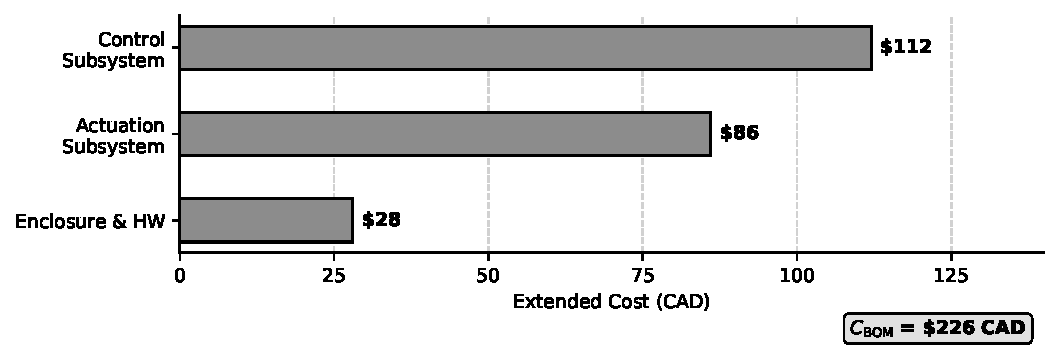
\includegraphics[width=0.80\textwidth]{images/fig_03_cost_rollup}
  \caption{BOM cost rollup by subsystem for the IoT robotic sorting subsystem.
           Horizontal bars show the contribution of each subsystem to the
           $C_{\text{BOM}} = \$124.85$~CAD total.
           Actuation dominates at \$77.35 (62\,\%), driven primarily by the
           gear motor (M1 at \$54.95).
           Control contributes \$42.55 (34\,\%) and Structure \$4.95 (4\,\%).}
  \label{fig:ch11-cost-rollup}
\end{figure}

\subsection{Overage Application}
\label{sec:ch11-worked-overage}

Applying $\alpha = 0.10$ (10\,\% overage) using Equation~\ref{eq:ch11-order-qty}
to the consumable and passive line:

\begin{enumerate}
  \item[(a)] H1 (enclosure hardware kit, fasteners) --- $q_{\text{H1}} = 1$,
        $q_{\text{H1}}^{\text{order}} = \lceil 1.10 \times 1 \rceil = \lceil 1.10 \rceil = 2$

The hardware kit is the only line where overage applies in this BOM: the
electronic modules are ordered to exact quantity (1 each), and one spare unit
is noted separately in the risk register rather than inflating the BOM cost.
The purchase list therefore shows H1 at quantity~2 ($2 \times \$4.95 = \$9.90$)
while the BOM cost calculation retains $q_{\text{H1}} = 1$,
$\text{ext}_{\text{H1}} = \$4.95$.
\end{enumerate}

\subsection{Supplier Quote Comparison: MQTT Radio Module (U2)}
\label{sec:ch11-worked-quote}

Two distributors were asked to quote the ESP-WROOM-32U at quantity~1.

\begin{table}[htbp]
  \centering
  \caption{Supplier quotes for U2 (ESP-WROOM-32U, Qty~1).
           All prices in CAD including applicable taxes and standard shipping
           to the lab address.}
  \label{tab:ch11-quote}
  \begin{tabular}{lrrp{4.5cm}}
    \toprule
    \textbf{Supplier}   & \textbf{Unit price (CAD)} & \textbf{Lead time} &
    \textbf{Notes} \\
    \midrule
    Mouser Electronics  & \$8.75  & 5 business days  & In stock (427 units); standard shipping included \\
    DigiParts CA        & \$7.90  & 14 business days & Ships from overseas warehouse; no local stock \\
    \bottomrule
  \end{tabular}
\end{table}

DigiParts CA offers a unit price \$0.85 lower than Mouser.
However, the lead time of 14 business days (approximately three calendar weeks)
places delivery after the assembly milestone on the Gantt chart from Chapter~10.
Missing that milestone delays Gate~3 by at least two weeks.

\textbf{Preferred choice: Mouser Electronics.}
The \$0.85 price advantage of DigiParts CA is outweighed by the lead-time risk.
At a project cost of \$124.85 per unit, the \$0.85 saving represents 0.7\,\%
of BOM cost --- an amount that is not worth delaying the project for.

\noindent The general procurement principle this illustrates: \emph{lead time is a schedule input, not a footnote}.
Any supplier whose lead time threatens a milestone date must be disqualified
regardless of unit price, unless the project manager explicitly approves the
schedule extension.

\paragraph{Common Pitfalls.}
The four most common BOM and procurement errors on prototype projects are:

\begin{enumerate}
  \item[(a)] \textbf{BOM as an afterthought.}\index{BOM!as afterthought}
        Starting the BOM after assembly begins means ordering parts under time
        pressure, paying expedite fees, and finding missing parts only when
        a build step stalls.
        The BOM should be started during architecture (Chapter~5) and completed
        before procurement begins.

  \item[(b)] \textbf{No alternates listed.}\index{alternate part!missing}
        A BOM with no alternate part column is a single-sourced BOM.
        When the preferred part is out of stock --- which happens routinely with
        popular ICs --- the project stalls while the team qualifies an alternate
        under pressure.

  \item[(c)] \textbf{Missing reference designators.}\index{reference designator!missing}
        Ordering a part without confirming the footprint against the reference
        designator on the PCB has no recovery path except rework or board
        respins.
        The reference designator column in the BOM is the link between the
        procurement document and the assembly drawing.

  \item[(d)] \textbf{Single-sourced parts with no risk register entry.}
        A component that can only be purchased from one supplier, with no
        qualified alternate and no risk register entry flagging the exposure,
        is an unmanaged risk.
        Every single-source line in the BOM should have a corresponding risk
        register entry with a mitigation (order extra stock, qualify an
        alternate before production).
\end{enumerate}

% ─────────────────────────────────────────────────────────────────────────────
\section*{Try It Yourself}
\label{sec:ch11-try}
% ─────────────────────────────────────────────────────────────────────────────

Your team is prototyping a battery-powered environmental sensor node.
The design BOM has six line items (one assembly unit):

\begin{table}[htbp]
  \centering
  \caption{Design BOM for the environmental sensor node (Try It Yourself).
           Unit costs in CAD at single-unit pricing.}
  \label{tab:ch11-try-bom}
  \begin{tabular}{llrrl}
    \toprule
    \textbf{Ref} & \textbf{Description / MPN}      & \textbf{Qty} &
    \textbf{UC (CAD)} & \textbf{Supplier} \\
    \midrule
    U1 & ATSAMD21G18A-MU MCU                      & 1 &  6.30 & Digi-Key \\
    U2 & RFM95W LoRa radio module                 & 1 &  9.45 & Mouser   \\
    U3 & BME680 environmental sensor              & 1 &  7.20 & Digi-Key \\
    BT1 & 18650 Li-ion cell (2500~mAh)            & 2 &  4.80 & BatterySpace \\
    C1  & 100~\textmu F electrolytic cap (assorted) & 5 &  0.30 & Digi-Key \\
    H1  & Enclosure + mounting hardware           & 1 &  8.75 & Amazon CA \\
    \bottomrule
  \end{tabular}
\end{table}

\begin{enumerate}
  \item Calculate the extended cost for each of the six lines using
        Equation~\ref{eq:ch11-ext}.
  \item Calculate $C_{\text{BOM}}$ using Equation~\ref{eq:ch11-bom-total}.
  \item Apply an overage of $\alpha = 0.15$ (15\,\%) to the capacitor line
        (C1) only, using Equation~\ref{eq:ch11-order-qty}.
        What is $q_{\text{C1}}^{\text{order}}$?
  \item A second supplier quotes the RFM95W at \$8.10 CAD but with a lead time
        of 18 business days (your assembly milestone is in 10 business days).
        Identify the preferred supplier and justify your choice using both unit
        price and lead time criteria.
  \item List two fields this BOM is missing that would be required for a
        Gate~3 submission.
\end{enumerate}

% ─────────────────────────────────────────────────────────────────────────────
\section*{Review Questions}
\label{sec:ch11-review}
% ─────────────────────────────────────────────────────────────────────────────

\begin{enumerate}
  \item \textbf{(Conceptual)} Explain the difference between a BOM and a
        purchase list.
        Under what circumstances does a purchase list differ from the BOM in
        both line count and quantity per line?

  \item \textbf{(Conceptual)} Why is an as-built BOM required even when the
        assembled unit matches the design BOM exactly?
        What does the as-built BOM provide that the design BOM does not?

  \item \textbf{(Applied)} A BOM has a line item for 0.1~\textmu F MLCC
        capacitors with $q = 12$ and $u = \$0.08$~CAD.
        \begin{enumerate}
          \item[(a)] Calculate the extended cost using
                Equation~\ref{eq:ch11-ext}.
          \item[(b)] Calculate the order quantity with $\alpha = 0.10$ using
                Equation~\ref{eq:ch11-order-qty}.
        \end{enumerate}

  \item \textbf{(Applied)} A BOM has five line items with extended costs of
        \$24.50, \$67.00, \$8.40, \$13.75, and \$5.90 (all CAD).
        Calculate $C_{\text{BOM}}$ using Equation~\ref{eq:ch11-bom-total} and
        identify which single line contributes the greatest fraction of total
        cost.

  \item \textbf{(Multi-step)} Supplier A quotes a microcontroller at
        \$11.20~CAD with a 4-business-day lead time and 50 units in stock.
        Supplier B quotes the same MPN at \$9.85~CAD with a 12-business-day
        lead time and 200 units in stock.
        Your assembly milestone is 7 business days from today and you need
        3 units.
        \begin{enumerate}
          \item[(a)] Calculate the total cost from each supplier for 3 units.
          \item[(b)] Identify the preferred supplier with explicit reasoning
                that addresses both price and schedule.
          \item[(c)] Describe one scenario in which the higher-priced supplier
                would \emph{not} be preferred despite meeting the schedule.
        \end{enumerate}
\end{enumerate}

% ─────────────────────────────────────────────────────────────────────────────
\section*{End-of-Chapter Artifact}
\label{sec:ch11-artifact}
% ─────────────────────────────────────────────────────────────────────────────

The Gate~3 deliverable from this chapter is a procurement package consisting
of three documents submitted together:

\begin{enumerate}
  \item[(a)] \textbf{Costed BOM}: all fields populated (reference designator,
        MPN, description, quantity, unit cost, extended cost, preferred
        supplier, distributor part number, lead time, alternate part).

  \item[(b)] \textbf{Purchase list}: one row per unique MPN with order
        quantities reflecting overage where applicable, derived from the BOM
        as described in Section~\ref{sec:ch11-purchase-list}.

  \item[(c)] \textbf{Procurement records}: for completed purchases, the set of
        POs, packing slips, and invoices with the three-way match completed;
        for pending purchases at Gate~3 submission, the set of accepted quotes
        and issued POs.
\end{enumerate}

A Gate~3 reviewer who cannot find a unit cost, a lead time, or an alternate
part for any line item in the costed BOM will flag the submission as incomplete.
The BOM is a design document; an incomplete design document is not ready for
review.

% ─────────────────────────────────────────────────────────────────────────────
\section*{Chapter Summary}
\label{sec:ch11-summary}
% ─────────────────────────────────────────────────────────────────────────────

The bill of materials functions as a design document: its completeness is a precondition for Gate~3 approval, not a post-assembly record.
It records the full set of physical parts needed for one assembled unit ---
reference designators, MPNs, quantities, unit costs, extended costs, supplier
information, lead times, and alternate parts --- and makes the cost and
supply-chain risk of the design visible to every reviewer.
The \textbf{extended cost} for each line is $\text{ext}_i = q_i \times u_i$
(Equation~\ref{eq:ch11-ext}).
The \textbf{BOM total} is $C_{\text{BOM}} = \sum q_i \times u_i$
(Equation~\ref{eq:ch11-bom-total}).
Order quantities for consumables are padded by an overage factor $\alpha$ using
$q_i^{\text{order}} = \lceil (1+\alpha)\,q_i \rceil$
(Equation~\ref{eq:ch11-order-qty}), but overage belongs only on the purchase
list --- never in the BOM cost calculation.

Supplier selection weighs unit price, lead time, stock availability, MOQ, and
shipping; the cheapest quote is not always the correct choice when lead time
threatens a Gantt milestone.
The procurement document chain --- BOM, purchase list, RFQ, PO, packing slip,
invoice, three-way match, as-built BOM --- provides traceability from design
intent to physical assembly and closes out the procurement budget with a
recorded variance.

You now have a costed BOM, a purchase list, and a set of procurement records.
Chapter~12 takes $C_{\text{BOM}}$ as its starting point and asks what happens to unit cost when the design scales from one prototype to low-volume production --- identifying the cost-reduction leverage points a Gate~4 reviewer will require.
